\documentclass[11pt, titlepage]{article}
\usepackage{amsmath,amsthm,amssymb}
\usepackage{hyperref, pgf, tikz}
\usepackage{fancyhdr}
\usetikzlibrary{arrows}
\usepackage[margin=1.25in]{geometry}
\usepackage{graphicx}                     
\pagestyle{fancy}
\usepackage{array}
%\usepackage{wrapfig}

\lhead{Lab \#7}
\rhead{\thepage}
\cfoot{}

\title{Conservation of Energy\\ \ \\ \large Lab \#7}
\author{Name: Avery Karlin \\ Partner: Nicholas Yang}
\date{}
\begin{document}

\maketitle

\begin{center}
\LARGE Conservation of Energy
\end{center}

\section*{Objective}
The objective of the lab is to measure the spring potential energy of a spring cart, and measure the maximum gravitational potential of the cart to determine if the energy is conserved.

\section*{Introduction}
The potential energy of a spring, $PE_{spring} = \frac{1}{2}kx^2$, such that the maximum spring potential energy is when x = A, compressed fully. The change in gravitational potential energy ($\delta PE_{g}$) is proportional to the change in height of the body, such that $PE_{g} = mg\delta h$. Conservation of mechanical energy states that mechanical energy is constant within a body acted on by conservative forces, such as spring and gravitational force, only changing form. Thus, $$\frac{1}{2}kx^2 = mg\delta h.$$

\section*{Procedures and Results}
First, we placed the cart with the spring not compressed on the track, after setting up the track such that it was level. We then placed a barrier on one side, with the pulley on the other side from the cart, and attached a string with different amounts of mass over the pulley, to measure the amount the cart's spring is compressed to find the spring constant.

Next, we elevated the track to a specific angle, found by measuring the height of the raised side, using the formula $\theta = sin^{-1}(\frac{h}{d})$, where d is the length of the platform, propelling the spring car, and measuring the distance along the platform it moved, using the same formula to find the height. We performed the test five times, and used the maximum height, to eliminate issues with the spring decompression. We then changed the mass of the cart, performing the same test, and changed the angle of the platform, performing the same test again.

\begin{figure}[p]
\centering
\hspace*{-10.5cm}
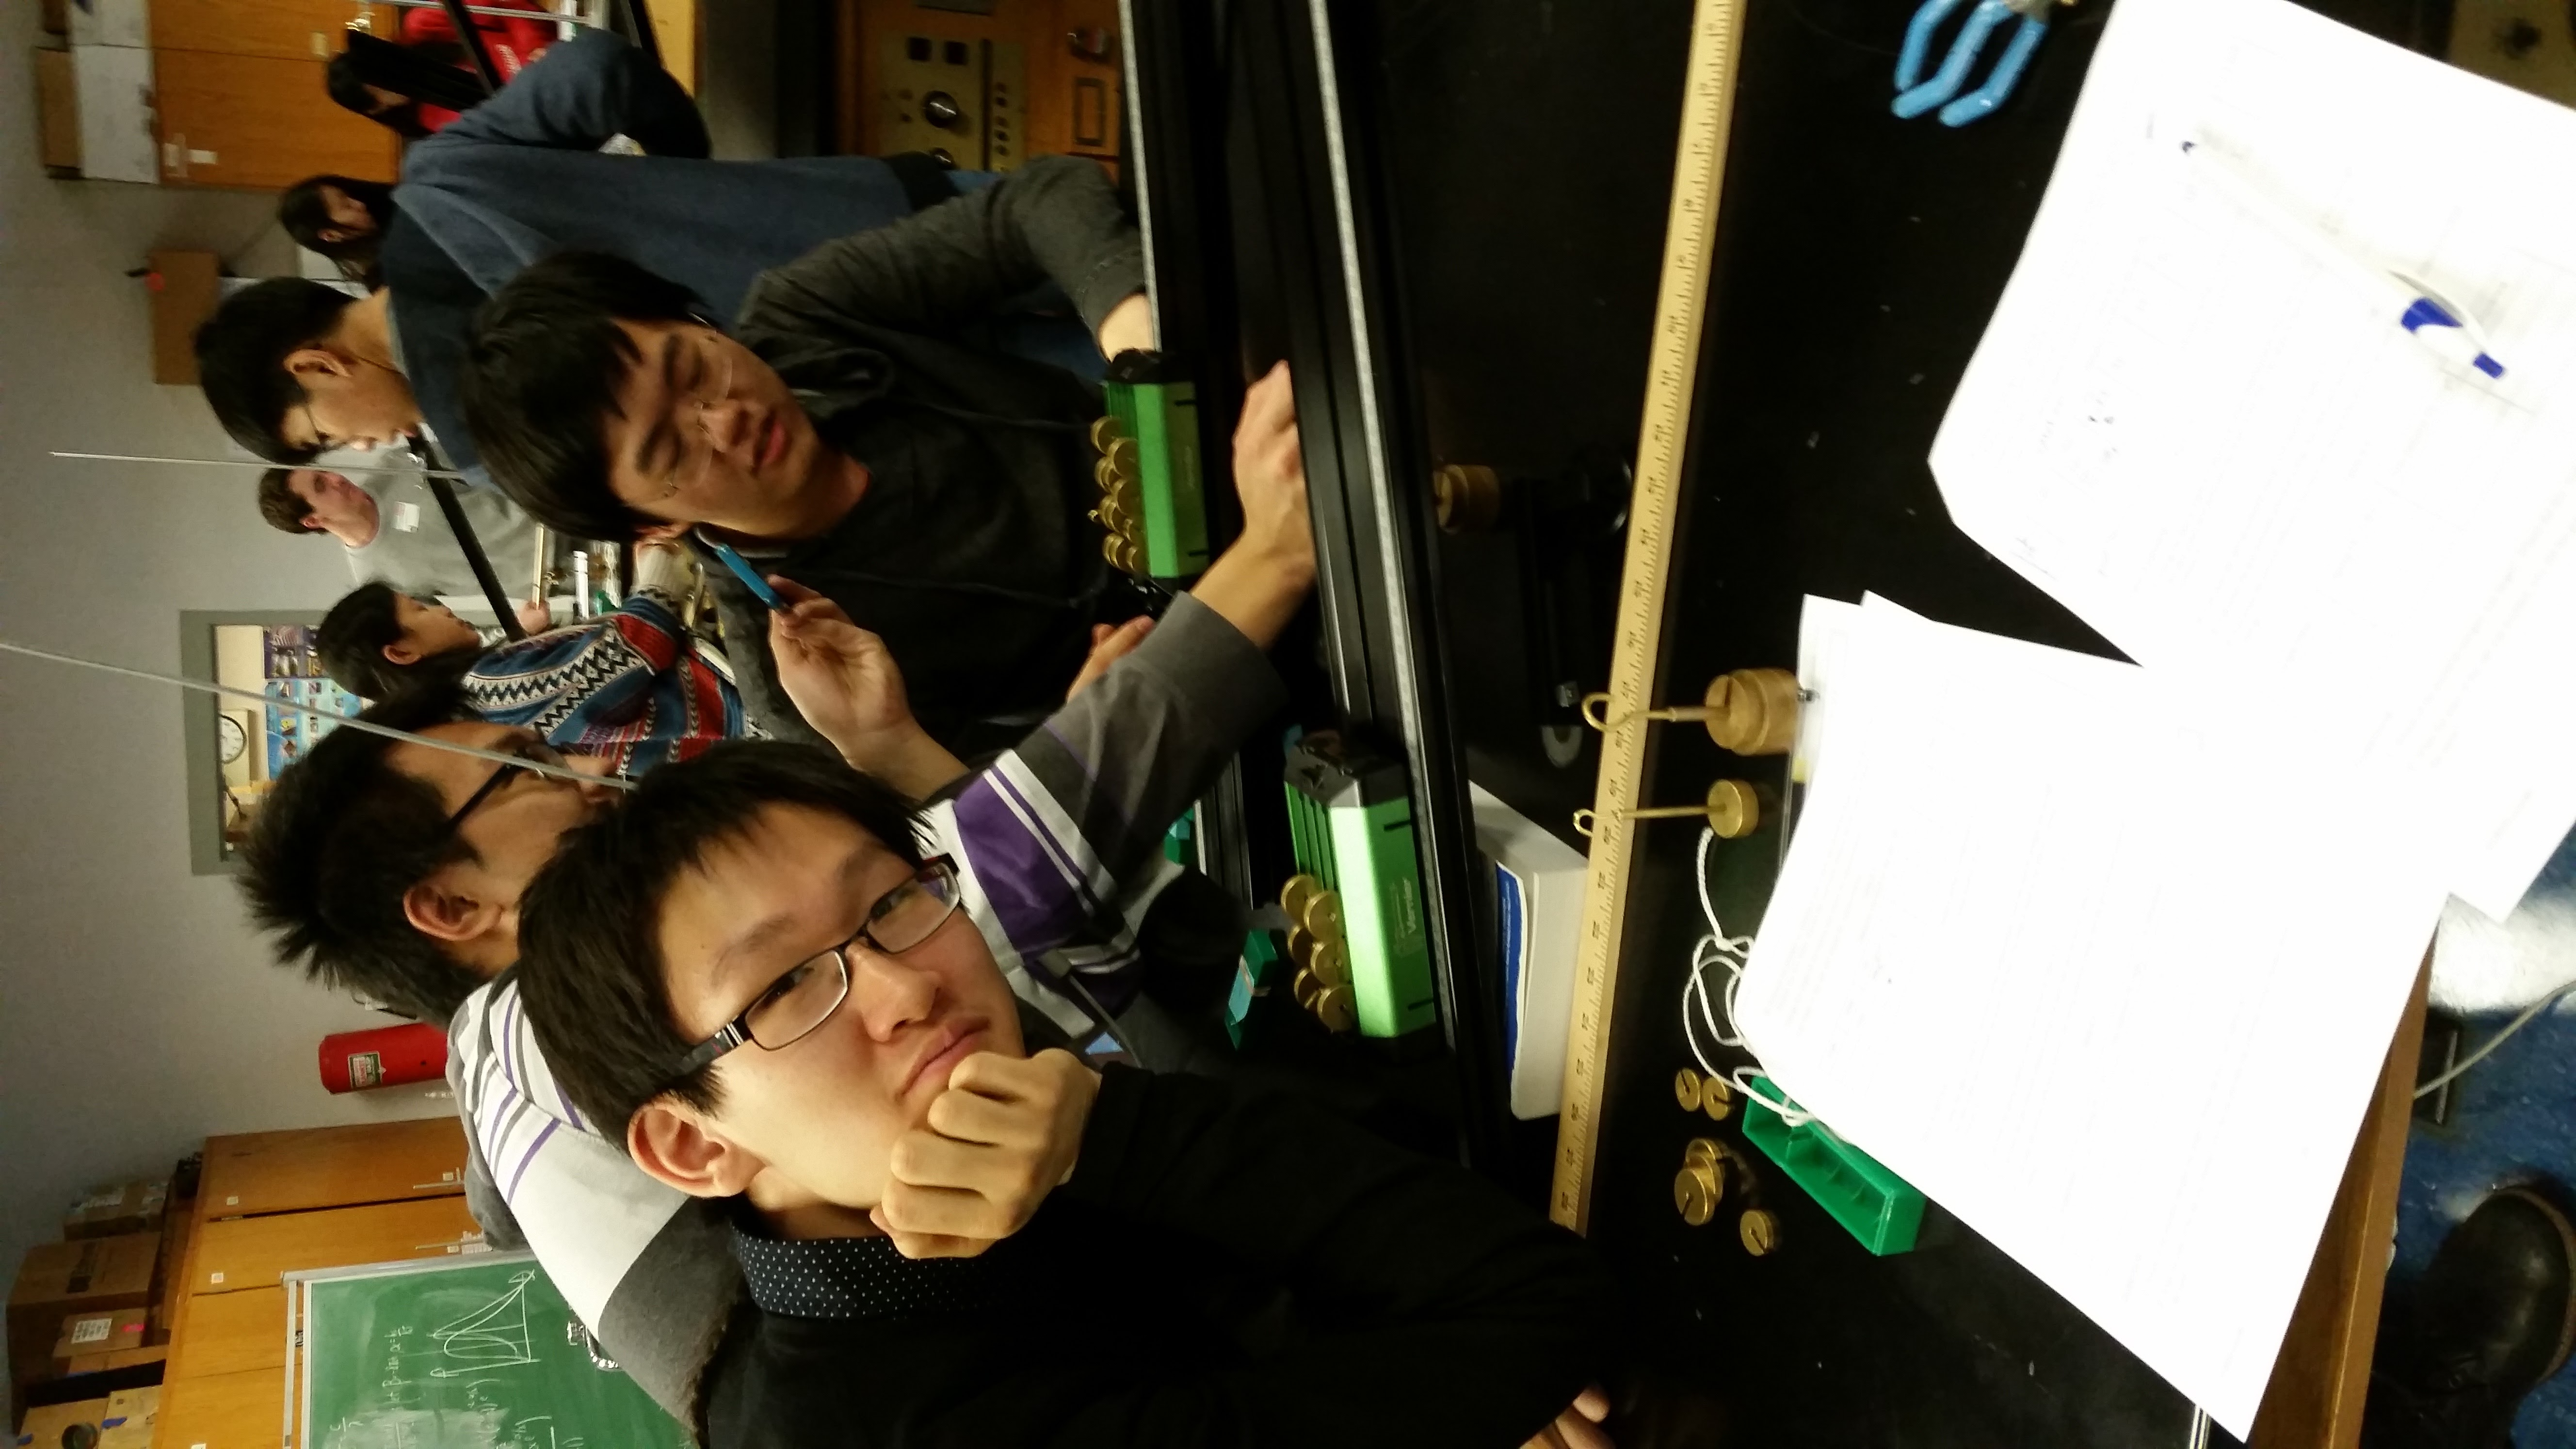
\includegraphics[scale=0.15, angle=270]{lab7.jpg}
\vspace*{19cm}
\end{figure}

\begin{center}
\begin{tabular}
{|m{15em}|m{15em}|}
Added Mass (kg) & Rear Cart Position (m) \\
0 & 0.231 \\
0.25 & 0.231 \\
0.5 & 0.231 \\
1.25 & 0.227 \\
1.5 & 0.215 \\
1.75 & 0.2135 \\
\end{tabular}

\begin{tabular}
{|m{5em}|m{5em}|m{5em}|m{5em}|m{5em}|m{5em}|m{5em}|}
Platform Height (m) & Mass (kg) & Trial 1 Rear Position (m) & 2 & 3 & 4 & 5 \\
0.28 & 0.5093 & 0.495 & 0.51 & 0.51 & 0.51 & 0.5 \\
0.36 & 0.5093 & 0.42 & 0.435 & 0.433 & 0.432 & 0.43 \\
0.28 & 0.6293 & 0.445 & 0.43 & 0.45 & 0.425 & 0.45 \\
\end{tabular}
\end{center}

\section*{Discussion}
Sample calculations for the non-measured data are as shown:

\begin{center}
\begin{tabular}
{|m{8em}|m{8em}|m{8em}|m{8em}|}
\end{tabular}
\end{center}

\section*{Conclusion}

\end{document}
